\section{Schleifen}

\begin{frame}{Schleifen}
\begin{itemize}
	\item for-Schleife
	\item while-Schleife
\end{itemize}
\end{frame}


\begin{frame}[fragile]{Hello World}
\textbf{Aufgabe 1}\\
	Erweitere das Programm so, dass  der \texttt{String} ''Hello World''
	6-mal ausgegeben wird.

\pause{}
\begin{exampleblock}{Lösung}
	\begin{lstlisting}
print("Hello World!")
print("Hello World!")
print("Hello World!")
print("Hello World!")
print("Hello World!")
print("Hello World!")
	\end{lstlisting}
\end{exampleblock}
\end{frame}

\begin{frame}{for-Schleife}
\centering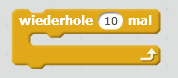
\includegraphics[scale=1.0]{images/for}
\end{frame}


\begin{frame}[fragile]{for-Schleife}
	Umgangssprachlich: \\
	Eine Variable (kann ein Buchstabe oder Wort sein) nimmt den Anfangswert an und erhöht sich pro Schleifendurchlauf um 1, solange die Variable \texttt{<} Ende. (Sie durchläuft alle Elemente in der range)
	
	\begin{lstlisting}
	for Variable in range(Anfang, Ende):
		# Programmcode
	\end{lstlisting}
	
	\begin{lstlisting}
		for i in range(1,7):
			print("Hello World!)
	\end{lstlisting}	
\end{frame}

\begin{frame}[fragile]{for-Schleife Übungen}
Verändere den Code so, dass ...
\begin{itemize}
\item Aufgabe 1: ...nur dreimal ''Hello World!'' ausgegeben wird\\
\item Aufgabe 2: ...nach jedem der 3 ''Hello World!'' ein ''Hello'' ausgegeben wird
\end{itemize}
\end{frame}


\begin{frame}[fragile]{Verwendung des Parameters im Code}
\textbf{Aufgabe}\\
    Schreibe ein Programm, das von 1 bis 100 zählt.\\
   1, 2, 3, .....

\begin{exampleblock}{Lösungsvariante 1}
    \begin{lstlisting}
	print(1)
	print(2)
	print(3)
	print(4)
	print(5)
	print(6)
	print(7)
	...
    \end{lstlisting}
    \pause{}
    \begin{lstlisting}
    for i in range(1, 101):
    	print(i)
    \end{lstlisting}
\end{exampleblock}
\end{frame}

\begin{frame}[fragile]{Aufgaben zu for-Schleifen}
Verändere den Code so, dass...
\begin{itemize}
	\item Aufgabe 1: nur Zahlen zwischen 35 und 40 ausgegeben werden
	\item Aufgabe 2: die Quadratzahlen für 1 bis 4 ausgegeben werden 
\end{itemize}
\end{frame}




